%%%%%%%%%%%%%%%%%%%%%%%%%%%%%%%%%%%%%%%%%
% Short Sectioned Assignment LaTeX Template Version 1.0 (5/5/12)
% This template has been downloaded from: http://www.LaTeXTemplates.com
% Original author:  Frits Wenneker (http://www.howtotex.com)
% License: CC BY-NC-SA 3.0 (http://creativecommons.org/licenses/by-nc-sa/3.0/)
%%%%%%%%%%%%%%%%%%%%%%%%%%%%%%%%%%%%%%%%%

% \documentclass[paper=a4, fontsize=11pt]{scrartcl} % A4 paper and 11pt font size
\documentclass[11pt, a4paper]{book}
\usepackage[T1]{fontenc} % Use 8-bit encoding that has 256 glyphs
\usepackage[utf8]{inputenc}
\usepackage{fourier} % Use the Adobe Utopia font for the document - comment this line to return to the LaTeX default
\usepackage{listings} % para insertar código con formato similar al editor
\usepackage[spanish, es-tabla]{babel} % Selecciona el español para palabras introducidas automáticamente, p.ej. "septiembre" en la fecha y especifica que se use la palabra Tabla en vez de Cuadro
\usepackage{url} % ,href} %para incluir URLs e hipervínculos dentro del texto (aunque hay que instalar href)
\usepackage{graphics,graphicx, float} %para incluir imágenes y colocarlas
\usepackage[gen]{eurosym} %para incluir el símbolo del euro
\usepackage{cite} %para incluir citas del archivo <nombre>.bib
\usepackage{enumerate}
\usepackage{hyperref}
\usepackage{graphicx}
\graphicspath{{figures/}}
\usepackage{tabularx}
\usepackage{booktabs}

\usepackage[table,xcdraw]{xcolor}
\hypersetup{
	colorlinks=true,	% false: boxed links; true: colored links
	linkcolor=black,	% color of internal links
	urlcolor=cyan		% color of external links
}
\renewcommand{\familydefault}{\sfdefault}
\usepackage{fancyhdr} % Custom headers and footers
\pagestyle{fancyplain} % Makes all pages in the document conform to the custom headers and footers
\fancyhead[L]{} % Empty left header
\fancyhead[C]{} % Empty center header
\fancyhead[R]{Antonio Gámiz Delgado} % My name
\fancyfoot[L]{} % Empty left footer
\fancyfoot[C]{} % Empty center footer
\fancyfoot[R]{\thepage} % Page numbering for right footer
%\renewcommand{\headrulewidth}{0pt} % Remove header underlines
\renewcommand{\footrulewidth}{0pt} % Remove footer underlines
\setlength{\headheight}{13.6pt} % Customize the height of the header

\usepackage{titlesec, blindtext, color}
\definecolor{gray75}{gray}{0.75}
\newcommand{\hsp}{\hspace{20pt}}
\titleformat{\chapter}[hang]{\Huge\bfseries}{\thechapter\hsp\textcolor{gray75}{|}\hsp}{0pt}{\Huge\bfseries}
\setcounter{secnumdepth}{4}
\usepackage[Lenny]{fncychap}
\usepackage{amsmath, amssymb}
\usepackage{amsthm}
\usepackage{tikz}
\theoremstyle{definition}
\newtheorem{definition}{Definición}[section]
\graphicspath{{figures/}}

\begin{document}

% \begin{titlepage}
\newlength{\centeroffset}
\setlength{\centeroffset}{-0.5\oddsidemargin}
\addtolength{\centeroffset}{0.5\evensidemargin}
\thispagestyle{empty}

\noindent\hspace*{\centeroffset}\begin{minipage}{\textwidth}

\centering

\includegraphics[width=0.9\textwidth]{logos/logo_ugr.jpg}\\[1.4cm]

\textsc{ \Large TRABAJO FIN DE GRADO\\[0.2cm]}
\textsc{ GRADO EN INGENIERIA INFORMATICA Y MATEMATICAS}\\[1cm]

{\Huge\bfseries Any2Vec \\}
\noindent\rule[-1ex]{\textwidth}{3pt}\\[3.5ex]
{\large\bfseries }
\end{minipage}

\vspace{2.5cm}
\noindent\hspace*{\centeroffset}
\begin{minipage}{\textwidth}
\centering

\textbf{Autor}\\ {Antonio Gámiz Delgado}\\[2.5ex]
\textbf{Director}\\ {Juan Julián Merelo Guervos \\ Serafín Moral Callejón }\\[2cm]

\includegraphics[width=0.3\textwidth]{logos/etsiit_logo.png}\\[0.1cm]
\textsc{Escuela Técnica Superior de Ingenierías Informática y de Telecomunicación}\\
\textsc{---}\\
Granada, Junio de 2022
\end{minipage}
\end{titlepage}

% \thispagestyle{empty}

\begin{center}
{\large\bfseries Any2Vec \\ Embddeddings para búsqueda de semántica y aritmética de contenidos no verbales }\\
\end{center}
\begin{center}
Antonio Gámiz Delgado \\
\end{center}

%\vspace{0.7cm}

\vspace{0.5cm}
\noindent{\textbf{Palabras clave}: \textit{software libre}
\vspace{0.7cm}

\noindent{\textbf{Resumen}\\


\cleardoublepage

\begin{center}
	{\large\bfseries Any2Vec \\ Embddeddings for semantic earch and non-verbal content arithmetic}\\
\end{center}
\begin{center}
	Antonio Gámiz Delgado\\
\end{center}
\vspace{0.5cm}
\noindent{\textbf{Keywords}: \textit{open source}, \textit{floss}
\vspace{0.7cm}

\noindent{\textbf{Abstract}\\


\cleardoublepage

\thispagestyle{empty}

\noindent\rule[-1ex]{\textwidth}{2pt}\\[4.5ex]

D. \textbf{Juan Julián Merelo Guervos}, Profesor del Departamento de Arquitectura y Tecnología de Computadores y
D. \textbf{Serafín Moral Callejón}, Profesor del Departamento de Ciencia de Computadores e Inteligencia Artificial
\vspace{0.5cm}

\textbf{Informan:}

\vspace{0.5cm}

Que el presente trabajo, titulado \textit{\textbf{Any2Vec, Embddeddings para búsqueda de semántica y aritmética de contenidos no verbales}},
ha sido realizado bajo mi supervisión por \textbf{Antonio Gámiz Delgado}, y autorizo la defensa de dicho trabajo ante el tribunal
que corresponda.

\vspace{0.5cm}

Y para que conste, expiden y firman el presente informe en Granada a Junio de 2022.

\vspace{1cm}

\textbf{El/la director(a)/es: }

\vspace{5cm}

\noindent \textbf{Juan Julián Merelo Guervos, Serafín Moral Callejón}

\chapter*{Agradecimientos}






% \newpage
% \tableofcontents

% \newpage
% \listoffigures

% \listoftables
% \newpage

\chapter{Introducción}

Un tropo, como describe Rizzo Michael \cite{rizzo2013art}, es una imagen
universalmente reconocida, con varias capas de significado contextual que
crean un nueva metáfora visual. Un buen ejemplo, es el tropo \emph{I can
    explain} \cite{tropo:ICanExplain}, donde un caracter que se siente culpable,
reacciona a la aparición de una figura autoritaria diciendo: \emph{"Puedo
    explicarlo!"}, procediendo a explicar lo que sea que haya pasado. Este tropo ha
sido enormemente utilizado en una infinidad de situaciones en obras culturales
\cite{tropo:ICanExplain}, desde \emph{Iron Man} hasta la serie de animación
\emph{Digimon}.

Cada película, libro o teatro, está formado por una inmensa cantidad de tropos
y, en cierta medida, su trama es caracterizada por ellos. Esa misma
caracterización, motiva un gran interés en el estudio de estos tropos: cómo se
relacionan entre ellos, cómo de comunes son, qué implicaciones tiene que una
obra cultural presente un cierto conjunto de tropos, etc.

Ese estudio es la principal motivación de este trabajo. Dado un conjunto de
obras culturales y los tropos que aparecen en ellas, se quiere estudiar la
relación existente entre los tropos y su rating, para obtener el máximo \emph
{rating} posible. En particular, este trabajo se centra en el estudio de tropos
encontrados en películas.

El trabajo está organizado en diferentes bloques:

\begin{enumerate}
    \item Bloque I: se describe en detalle el problema que se trata en el
          trabajo, seguido del estado del arte en el uso del NLP para encontrar
          relaciones entre palabras. A continuación, se detalla la planificación
          seguida para resolver el problema, así como las prácticas seguidas para
          realizarla.
    \item Bloque II: desarrollo teórico de la base matemática usada para la
          realización de este trabajo.
    \item Bloque III: se describe el proceso de análisis e implementación
          llevados a cabo, así como unas conclusiones finales.
\end{enumerate}

Este proyecto es software libre, y está liberado con la licencia \cite{gplv3}.

\section*{Definiciones previas}

Antes de pasar a la descripción del problema, es necesario definir algunos conceptos importantes para
este trabajo.

\subsection*{\textit{Embeddings}}

En el análisis de datos de texto se suele encontrar el problema de la alta dimensionalidad de los datos. Por eso surgió el
Análisis Semántico Latente (o más conocido por LSA, \textit{Latent Semantic Analysis}), que es una técnica popular
de reducción de la dimensionalidad. Básicamente transforma datos en forma de texto en términos de $d\in\mathbb{N}$
características latentes (es decir, escondidas), donde $d<m$, siendo $m\in\mathbb{N}$, el número de términos en los
datos. Una de las primeras menciones del término \textit{embedding} puede ser encontrada en \cite{landauer1997learning}.
En este trabajo, un \textit{embedding} se va a definir como:

\begin{definition}[Embedding]
    Dado un conjunto de datos $D$, de tamaño $m\in\mathbb{N}$, un término $w\in D$, el embedding de $w$ es
    la representación en un vector de $d$ dimensiones (o características) con $d<m$.
\end{definition}

Este concepto puede ser usado para codificar la semántica de un término, en un espacio vectorial de dimensión reducida
y fija, $m$, de forma que se pueda operar con esas representaciones de forma sencilla y eficiente. A continuación se ve cómo
se deduce la semántica del término a partir de su \textit{embedding}. Normalmente si el conjunto de datos son palabras, el nombre
que se suele usar es \textit{word embedding}.

\subsection*{Semántica de un embedding}

La motivación para usar \textit{embeddings} con palabras proviene de la idea de John Rupert
Firth de que `una palabra se caracteriza por la compañía que mantiene' \cite{firth1957synopsis}. Por ejemplo, si no se sabe
el significado de la palabra \textit{coche}, pero aparece en las siguientes frases (o contextos):
\begin{itemize}
    \item El coche es muy importante para el transporte en las zonas rurales.
    \item En la autovía, la velocidad máxima de un coche son 120 kilómetros por hora.
    \item El coche y otros vehículos...
\end{itemize}
Y suponiendo que se han visto esas mismas palabras en otros contextos:
\begin{itemize}
    \item Un camión es usado para el transporte de grandes mercancías.
    \item Un camión no puedo alcanzar gran velocidad.
\end{itemize}
Del hecho de que \textit{coche} aparezca al lado de palabras como \textit{transporte}, \textit{velocidad} y \textit{vehículo},
de igual forma aparecen para camión, sugiere que un coche y un camión son similares (ambos son vehículos). Usando esta intuición,
ahora se va a introducir como detectar estas relaciones matemáticamente.


Dada una palabra, se puede generar un vector que represente el valor semántico de tal palabra (\textit{embedding}), es decir, qué significa la palabra, qué caracteriza
su significado, etc. Esta representación vectorial se genera de forma que se puedan obtener otras palabras
cercanas `semánticamente' (dada la representación vectorial de la palabra \textit{coche}, la representación de la palabra \textit{camión}
debería ser cercana semánticamente a la de camión porque ambas son vehículos). Para medir este concepto se va a definir una forma de medir el nivel
de cercanía semántica entre dos palabras. Una posible forma sería usar la similitud coseno (es importante notar que la similitud coseno no es una función de medida,
ya que no cumple la desigualdad de Schwarz):

\begin{definition}
  Dados dos vectores $a,b\in\mathbb{R}$, $n\in\mathbb{N}$, se define la similitud coseno como:
  \[
    S_c(a,b)=\cos\theta = \frac{a\cdot b}{\norm{a}\norm{b}} \in [-1, 1]
  \]
donde $\theta\in[-\pi,\pi]$ es el ángulo entre los vectores $a$ y $b$.
\end{definition}

Se usa esta función para medir la cercanía semántica porque la magnitud de los vectores usados para las representaciones no aporta
ningún valor semántico, sino que es la dirección del vector la que lo aporta. Sea un embedding de dimensión $d\in\mathbb{N}$, es decir,
se tienen $d$ componentes numéricas por cada embedding. El valor de las componentes (o más bien las combinaciones lineales) de esos embeddings,
codifican el significado semántico de cada palabra. Un famoso ejemplo de este cálculo sería \emph{rey} - \emph{hombre} + \emph{mujer} = \emph{reina} \cite{drozd-etal-2016-word}.
De ahí se puede deducir que hay una cierta dirección que más o menos apunta al concepto de realeza y otra dirección que apunta al concepto de género.

A partir de ese ejemplo, se puede ver perfectamente la razón de que la magnitud de los vectores no sea relevante pero sí lo sea su dirección. Sean $a,b\in\mathbb{R}^d$ dos embeddings
distintos, de forma que $a=(-1, 2, 3)$ y $b=(-3, 6, -9)$. Estos dos vectores tienen magnitudes totalmente distintas ($a=3b$), pero apuntan hacia la misma dirección
(por lo que tienen similitud coseno igual a 0, $S_c(a,b)=0$). Eso es el resultado esperable porque significa que tienen la misma proporción relativa en cada componente.
Sin embargo, si se hubiera usado la distancia euclídea usual, la distancia entra $a$ y $b$ sería de aproximadamente $7.48$. Sería fácil encontrar otro vector $c$ igual de cercano (distancia euclídea) a $a$
que $b$, pero probablemente apuntaría en una dirección totalmente distinta.

Con estos conceptos definidos, se puede definir el problema y ver el estado del arte en cuanto a la generación y uso de estos embeddings.
\chapter{Descripción del problema}

En este capítulo se va a expandir el problema que brevemente se ha comentado en
la introducción, así como los objetivos a resolver por este trabajo.

\section{Problema a resolver}

A la hora de crear una obra cultural, como una película, los guionistas de cine
tienen que crear una trama argumental. De forma ineludible, esa trama va a
estar caracterizada por un conjunto de tropos. Es interesante destacar, que la
guionista no tiene por qué ser consciente de los tropos que está usando, o incluso podría estar creando tropos nuevos, que serán usados por otros
escritores.

Esa incertidumbre, puede incitar las siguientes preguntas: ¿qué conjunto de
tropos funcionan bien juntos?, ¿hay conjuntos de tropos que no casen bien?,
¿qué combinación de tropos puedo usar para aumentar la probabilidad de éxito de
mi película? Seguramente cada guionista se haga esas preguntas mientras decide
si bromear sobre Adolf Hitler \cite{tropo:AdolfHitlarious} o introducir a unos
alienígenas que abducen vacas \cite{tropo:AliensStealCattle}.

Por lo tanto, el problema a resolver es el siguiente: dado un conjunto de
tropos, encontrar subconjuntos de tropos cuyo \emph{rating} sea máximo.

\section{Objetivos} \label{section:goals}

Una vez está claro el problema a resolver, se pueden enumerar los principales
objetivos del trabajo:

\begin{enumerate}
      \item Desarrollar una herramienta útil para que los guionistas puedan
            consultar una estimación del rating de los tropos de su guión.
      \item Permitir que la funcionalidad de este trabajo pueda ser integrada con
            el mayor número de clientes.
      \item Crear un proyecto extensible y de código abierto para que futuros
            contribuidores al trabajo puedan complementar el trabajo con otras obras
            culturales como libros o cómics.
\end{enumerate}
\chapter{Estado del arte}

El concepto de \emph{tropo} para el cine fue definido por Michael Rizzo \cite{rizzo2013art} en el año 2013. Este término
tiene el mismo origen que los tropos para la literatura, cuyo estudio y clasificación fue una importante investigación en el
campo de la retórica (como por ejemplo, el estudio de tropos en películas \cite{nelson1998tropes}). En el ámbito del cine,
los tropos han sido usados para el estudio de la semiología de las películas \cite{howtoreadafilm}, que inlcuye el estudio
de los signos o elemenos de una película y su significado (semántica).

Hay algunos estudios recientes sobre los tropos en películas \cite{garcia2018overview} que han ayudado a interpretar las
películas y los tropos que se encuentran dentro de ellas. En este trabajo se pretende extender ese estudio aplicando el uso
de \emph{embeddings}, para extraer más información sobre los tropos y su semántica.

La primera noción de \textit{embedding} proviene del concepto matemático de una instancia de alguna
estructura matemática contenida en otra. Como por ejemplo, los números naturales, contenidos en los números enteros
$\mathbb{N}$. Seguramente inspirado por este concepto, surgió el concepto de \textit{embedding} en la rama del procesamiento
del lenguaje natural.

A lo largo del tiempo, numerosos modelos han sido usados para encontrar o calcular estos \textit{embeddings}, cada uno
con una aproximación diferente. A continuación se ven algunos de estos modelos.

En el modelo \emph{word2vec} \cite{word2vec:1} \cite{word2vec:2}, se crea una representación
en forma de vector para cada palabra. El principal problema de este modelo es que cada palabra tiene un único vector asociado,
pero en el mundo real, cada palabra puede tener distintos significados dependiendo del contexto.
Por ejemplo, en las frases \emph{kiwi y mango son coches españoles}, y \emph{kiwi y mango son frutas},
el mismo word embedding es usado para kiwi y mango.

Modelos como \emph{Adaptive Skipgram} \cite{adaptiveskipgram}, intentan solventar este problema usando
varios vectores para \emph{cada} sentido de una palabra, generando así un vocabulario de sentidos de palabras.
Sin embargo, se sigue usando el mismo embedding para cada ocurrencia de un sentido en específico.

Entre los últimos avances se encuentra \emph{BERT/ELMO} \cite{bert}, un exitoso modelo que soluciona el
problema antes descrito. En lugar de aportar información sobre el significado de una palabra, se construye
un embedding dependiente del contexto (y por lo tanto, específico a cada aparición). De forma que la palabra
\emph{kiwi} tendrá diferentes embeddings en las frases \emph{kiwi y mango son coches españoles}, y
\emph{kiwi y mango son frutas}.

En el caso de este trabajo, los tropos no tienen, a priori, distintos sentidos, por lo que se ha optado
por usar el modelo \emph{word2vec}.

Como el nombre del trabajo indica, la intentación es generar \textit{any embeddings}, es decir, no solo aplicado a
palabras \cite{word2vec:1} \cite{word2vec:2} o frases \cite{kiros2015skip}. En este trabajo en particular, se va a centrar
el estudio en generar embeddings para tropos de películas.

\chapter{Planificación}

En este capítulo se detalla la planificación del proyecto y las metodologías y buenas prácticas
usadas para el desarrollo del mismo. Siguiendo uno los objetivos de este trabajo, la planificación
ha sido muy influenciada por el desarrollo ágil aplicado a la ciencia \cite{desarrolloagil}.

\section{Metodología utilizada}

\subsection{Kanban}

Como el objetivo del trabajo es \textit{ser ágil}, es necesario escoger una metodología de trabajo que
lo permita. En este proyecto se ha escogido \textit{Kanban}. Los objetivos principales de kanban son dar
visibilidad al trabajo que se está haciendo, maximizar la eficiencia y limitar la cantidad de trabajo
en progreso. Esto se hace a través de un tablero en el que de un simple vistazo, se puede consultar el
estado del trabajo.

Kanban se base en hacer pequeños cambios incrementales de forma que el esfuerzo para que se puede realizar
la tarea sea mínimo. Esto no implica que Kanban favorezca la rapidez sobre la calidad, al contrario,
prevalece la calidad del producto final sobre la velocidad de desarrollo.

\subsection{Desarrollo dirigido por pruebas}

Kanban es una metodología para organizar el trabajo. A la hora de escribir código, es necesario usar
buenas prácticas adicionales. El desarrollo dirigido por tests (TDD, del inglés \textit{Test Driven Development})
es un gran complemento a Kanban, ya que nos permite hacer incrementos pequeños que aporten valor al
producto final. El flujo de trabajo consiste en:

\begin{itemize}
    \item Escribir test: definir un test que comprueba que la nueva funcionalidad funciona como es debido.
          Evidentemente, al principio debe fallar (salir en rojo) porque no hay nada implementado.
    \item Implementar funcionalidad: escribir \textit{solo} el código necesario para hacer pasar el test
          (que salga en verde).
    \item Refactorizar: iterar sobre la solución obtenida para mejorarla.
\end{itemize}

\subsection{Github}

Para implementar lo enunciado anteriormente, el trabajo ha sido desarrollado usando \textit{git} y \textit{GitHub}.
Para ello, las tareas necesarias se han dividido en hitos \cite{milestones}. Cada hito contiene una
serie de \textit{issues}, o tareas a resolver, para alcanzar dicho hito.

Para implementar la tabla de Kanban también se ha usado Github, ya que implementa de forma nativa un
tablero que permite definir las columnas comunes en esta metodología:

\section{Usuarios}

Los usuarios o \textit{stakeholders} de este proyecto son:

\begin{enumerate}
      \item Tribunal: al ser un trabajo de fin de grado, el proyecto debe llevar asociado una memoria
            que explique el trabajo.
      \item Tutores: el trabajo esta cotutorizado por varias personas que no son expertas en ambas partes del trabajo.
      \item Científico de datos: investigador que quiera expandir este trabajo o usarlo como
            referencia en alguno de sus proyectos. Se asume que este usuario tiene alto conocimiento técnico.
      \item Guionista: profesional cuyo principal interés es modificar los tropos de su película para
            conseguir un buen rating. Se asume que este usuario no tiene, en principio, ningún conocimiento
            técnico.
\end{enumerate}

\section{Historias de usuario}

Una vez se conocen los usuarios del trabajo, se pueden desarrollar sus principales historias de usuario o casos de uso:

\subsection{[HU0] Configuración del proyecto} \label{uc:configuration}

Como tutores necesitamos disponer de una forma fácil de leer el resultado en cada
una de las iteraciones.

Como tribunal necesitamos disponer de una forma fácil de leer el resultado final.

\subsubsection{Criterios de aceptación}

\begin{itemize}
      \item Debe estar claro que metodología se está llevando a cabo para el desarrollo del trabajo.
      \item Se debe poder generar el trabajo de forma sencilla.
      \item Se debe incluir una sección en la que se detalle el estado del arte.
      \item Los objetivos e historias del usuario deben de estar definidos.
\end{itemize}

\subsection{[HU1] Análisis de tropos}

Como científico de datos necesito un modelo reproducible que pueda alimentar con mis propios
conjuntos de datos.

Como tribunal/tutor necesito ver el desarrollo matemático e informático necesario para realizar
un análisis semántico de los tropos para que pueda evaluar al estudiante.

En este primera iteración del trabajo los datos sobre \textit{rating} no se van a incluir para
hacer las historias de usuario más pequeñas e independientes (acorde a \textit{INVEST} \cite{buglione2013improving})

\subsubsection{Criterios de aceptación}

\begin{itemize}
      \item Dado un conjunto de tropos, se deben poder obtener sus representaciones para operar con ellos  (\textit{embeddings}).
      \item El desarrollo del algoritmo tiene que estar claramente explicado, incluyendo el desarrollo de las herramientas matemáticas usadas.
\end{itemize}


\subsubsection{[HU2 ]Primera extensión del modelo Word2Vec}\label{uc:word2vec_primera_extension}

Como tribunal/tutor/científico de datos
necesito entender cómo se ha extendido el modelo Word2Vec para analizar la semántica de un conjunto de
tropos. Este extensión debe permitir que el modelo acepte conjuntos de palabras (tropos) sin orden, ya
los tropos son conjuntos no ordenados.

\subsubsection{Criterios de aceptación}

\begin{itemize}
      \item La implementación de la extensión debe estar documentada.
      \item El desarrollo del algoritmo tiene que estar claramente explicado, incluyendo el desarrollo de las herramientas matemáticas usadas.
\end{itemize}

\section{Temporización}
\begin{itemize}
    \item Tareas por hacer
    \item En progreso
    \item Hechas
\end{itemize}

Además esto ha sido complementado con la herramienta de \textit{pull requests} de Github para poder hacer
un desarrollo incremental de forma cómoda.

\chapter{Redes neuronales}

Este trabajo gira en torno al algoritmo \textit{Word2Vec} \cite{word2vec:1} \cite{word2vec:2}, una técnica de procesamiento
de lenguaje natural, que usa \textit{aprendizaje profundo} para su funcionamiento. El aprendizaje
profundo es una rama del Aprendizaje Máquina, que a su vez está incluido dentro del campo más general
de la Inteligencia Artificial. En general, el objetivo del aprendizaje máquina es estudiar algoritmos
que mejoran a partir de la experiencia. Tom M. Mitchell \cite{mitchell1997} enunció una definición formal
del término:

\begin{definition}[Aprender]
    Se dice que un programa \textit{aprende} de una experiencia \textit{E}, con respecto a un grupo
    de tareas \textit{T} y una medida de rendimiento \textit{P}, si su rendimiento en las tareas de
    \textit{T}, medido por \textit{P}, mejora con la experiencia \textit{E}.
\end{definition}

Estas técnicas suelen estar basadas en el concepto biológico de redes neuronales, las cuales están formadas por neuronas. A lo largo de este capítulo, se va a formalizar este concepto de neurona y se va a definir cómo interactúan entre ellas.

\section{Introducción}

Las redes neuronales suelen ser usadas en objetos que, a priori, no tienen una representación matemática,
como imágenes. El procedimiento habitual es encontrar una representación numérica que permita, de forma
cómoda, operar con esos objetos. Por ejemplo, para representar una imagen en blanco y negro, se puede
tomar un vector $x$, con tantas entradas como píxeles, donde cada entrada es un valor entre 0 y 1,
representando el valor del color en ese píxel. La red neuronal ahora debe tomar ese valor de entrada,
y producir otra representación matemática distinta, que también debe ser interpretada. Por ejemplo,
si se quieren detectar números escritos en la imagen, la representación de salida puede ser un vector
de 10 entradas, donde el valor de cada entrada será igual a 1 si el índice de esa entrada coincide con
el número presente en la imagen.

\begin{figure}[H]
    \centering
    \begin{tikzpicture}[
            roundnode/.style={circle, draw=black, minimum size=7mm},
        ]

        \node[roundnode]   at (1,4)   (input2)  {$x_2$};
        \node[roundnode]   at (1,6)   (input1)  {$x_1$};
        \node[roundnode]   at (5,4)   (hidden2)  {};
        \node[roundnode]   at (5,6)   (hidden1)  {};
        \node[roundnode]   at (7,5)   (output)  {};

        \draw[-stealth] (input1) -- node[above,xshift=1cm]   {$w_1$} (hidden1);
        \draw[-stealth] (input2) -- node[above,xshift=1cm, yshift=-0.1cm]   {$w_2$} (hidden1);
        \draw[-stealth] (input1) -- node[above, xshift=1cm, yshift=-0.7cm] {$w_3$} (hidden2);
        \draw[-stealth] (input2) -- node[below, xshift=1cm]   {$w_4$} (hidden2);

        \draw[-stealth] (hidden1) -- node[above]   {$w_5$} (output);
        \draw[-stealth] (hidden2) -- node[below]   {$w_6$} (output);

        \draw[] (output) -- node[right, xshift=0.3cm] {$y$} (8,5);

    \end{tikzpicture}
    \caption{Ejemplo de red neuronal con una capa escondida}
    \label{redneuronal:1}
\end{figure}

\subsection{Conceptos iniciales}

Para a partir de un vector de entrada $x\in\mathbb{R}^n$, producir un vector de salida $v\in\mathbb{R}^m$,
con el resultado que se quiere, será necesario realizar ciertas operaciones entra cada una de las capas
de la red neuronal, como se muestra en la Figura \ref{redneuronal:1}. Cada una de estas operaciones, activará
algunas neuronas en cada capa, produciendo al final el vector deseado. Una neurona no es más ni menos
que un escalar, entre 0 y 1 normalmente, cuyo valor es calculado usando el valor de las neuronas de la
capa anterior (o del input, si es la segunda capa) junto con el valor de los pesos $w_i$:

\[
    a^{(n+1)} = a^{(n)}_1w^{(n)}_1+a^{(n)}_2w^{(n)}_2+\cdots+a^{(n)}_nw^{(n)}_n=\sum_{i=1}^na^{(n)}_iw^{(n)}_i\in\mathbb{R}
\]

Los pesos no son más que números arbitrarios, que son actualizados en cada fase de aprendizaje \cite{rumelhart1986learning}.
Es trivial comprobar que $a^{(n+1)}$ es un número real, de cualquier valor. Esto es problemático porque
lo que se quiere ahora es saber cuando una neurona está \textit{activa}. Para ello, se puede usar lo
que se denomina una \textit{función de activación}, que no es ni más ni menos que una función  que transforma
la recta real en el intervalo $[0,1]$. Intuitivamente, el valor que devuelve la función de activación dice
cómo de positivo es el valor de esa neurona. Hay muchas elecciones posibles de función de activación, a continuación
se proponen algunas.

\subsubsection{Sigmoide}

La función sigmoide está definida como:
\begin{align*}
    \sigma \colon & \mathbb{R} \longrightarrow ]0,1[             \\
    \quad         & x \longmapsto \sigma(x) = \frac{1}{1+e^{-x}}
\end{align*}

Esta función es una de las más usada como función de activación. Entre sus principales ventajas está que es diferenciable, monótona y regular. Además, tiene dos características que serán usadas posteriormente:
\begin{equation} \label{sigmoid:1}
    \sigma(-x)=1-\sigma(x)
\end{equation}
\begin{equation} \label{sigmoid:2}
    \frac{d\sigma(x)}{dx}=\sigma(x)\sigma(-x)
\end{equation}

\begin{figure}[H]
    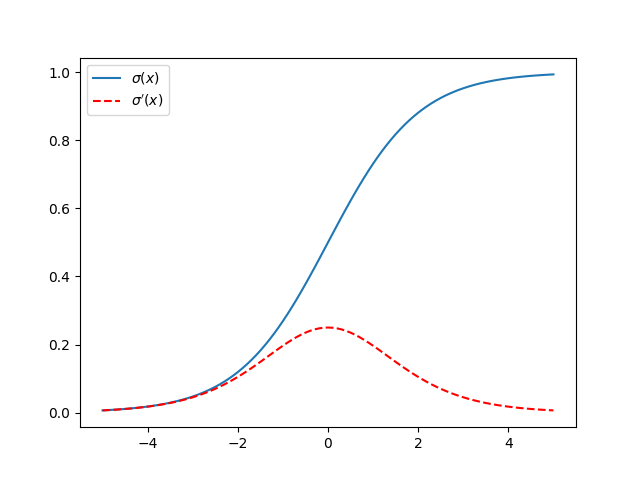
\includegraphics[width=7cm]{sigmoid.png}
    \centering
\end{figure}

El principal problema de esta función se denomina \textit{vanishing problem} \cite{hochreiter1991untersuchungen}.
Cuando se avance un poco más en los fundamentos de las redes neuronales, se volverá a este problema.

\subsubsection{Tangente Hiperbólica}

La función tangente hiperbólica está definida como:
\begin{align*}
    f \colon & \mathbb{R} \longrightarrow ]0,1[                       \\
    \quad    & x \longmapsto f(x) = \frac{e^{x}-e^{-x}}{e^{x}+e^{-x}}
\end{align*}

En el gráfico de esta función, se puede apreciar que su derivada es más pronunciada que la de la función sigmoide. Esto permite a la red neuronal aprender de forma más rápida, haciendo el aprendizaje más eficiente.

\begin{figure}[H]
    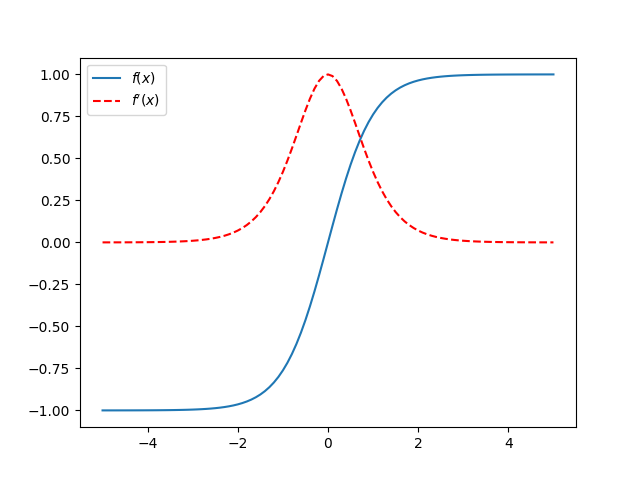
\includegraphics[width=7cm]{tanh.png}
    \centering
\end{figure}

\subsubsection{Unidad Linear Rectificada (ReLU)}

La función ReLU está definida por:
\begin{align*}
    f \colon & \mathbb{R} \longrightarrow ]0,1[ \
    \quad    & x \longmapsto f(x) = \max(0,x)
\end{align*}

Evidentemente, está función es mucho más eficiente, computacionalmente hablando, que las dos primeras alternativas. Sin embargo, presenta un gran problema: cuando los valores de entrada se aproximan o son inferiores a 0, la red no puede efectuar propagación hacia atrás, por lo que no puede aprender.

\begin{figure}[H]
    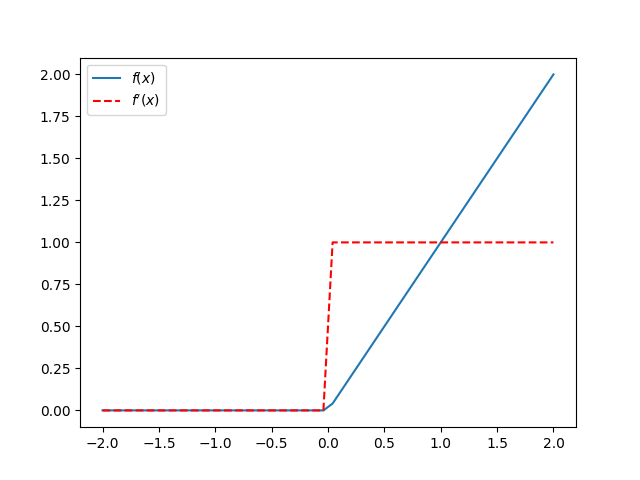
\includegraphics[width=7cm]{relu.png}
    \centering
\end{figure}


Por lo tanto, después de este razonamiento, el valor de cada neurona se calculará siguiendo la expresión:

\begin{equation}
    \label{eqn:1}
    a^{(n+1)}_j = f\left( b^{(n)}_j + \sum_{i=1}^n a^{(n)}_i w^{(n)}_i \right) \in [0,1]
\end{equation}

donde $b^{(n)}$ es otro valor arbitrario que va siendo actualizado para modificar el valor de salida de la
función de activación $f$.

\subsection{Notación}

Las redes neuronales suelen ser más complejas que la expuesta en la Figura \ref{redneuronal:1}. Normalmente,
se tienen muchos más inputs, pesos y capas escondidas. Por esa razón, una notación matricial para describir
las operaciones que se van a realizar es bastante adecuada. Como se verá en el siguiente capítulo, nuestra
red neuronal de interés solo tiene una capa escondida, así que se adaptará la notación a ese hecho:

\begin{itemize}
    \item Los subíndices $k$, $i$ y $j$ serán usados para denotar los valores de entrada, los valores de la
          capa escondido y los valores de salida, respectivamente.
    \item $x_1, \ldots x_K$ es el vector con los valores de entrada.
    \item $h_1, \ldots h_N$ es el vector con los valores de la capa escondida.
    \item $y_1, \ldots y_M$ es el vector con los valores de salida.
    \item $W = (w_{ki})$ es una matriz de dimensiones $n\times m$, donde $n$ es la dimensión
          del vector de entrada, $m$ la dimensión del vector de valores de la capa escondida y $w_{ki}$ es el peso de la conexión de la
          neurona $x_k$ con la neurona $h_i$.
    \item $W' = (w_{ij}')$ es una matriz de dimensiones $m\times q$, donde $m$ es la dimensión
          del vector de valores de la capa escondida, $q$ es la dimensión del vector de salida y $w_{ki}'$
          es el peso de la conexión de la neurona $h_i$ con la neurona $y_j$.
\end{itemize}

\begin{figure}[H]
    \centering
    \begin{tikzpicture}[
            roundnode/.style={circle, draw=black, minimum size=3mm},
        ]

        \node[] at (0,5) {Entrada};
        \node[] at (3,5) {Capa escondida};
        \node[] at (6,5) {Salida};

        \node[roundnode]   at (0,0)   (inputK)  {$x_K$};
        \node[roundnode]   at (0,2)   (input3)  {$x_3$};
        \node[roundnode]   at (0,3)   (input2)  {$x_2$};
        \node[roundnode]   at (0,4)   (input1)  {$x_1$};

        \path (input3) -- (inputK) node [black, font=\Huge, midway, sloped] {$\dots$};

        \node[roundnode]   at (3,0.5)   (hiddenN)  {$h_N$};
        \node[roundnode]   at (3,2.5)   (hidden2)  {$h_2$};
        \node[roundnode]   at (3,3.5)   (hidden1)  {$h_1$};

        \path (hidden2) -- (hiddenN) node [black, font=\Huge, midway, sloped] {$\dots$};

        \node[roundnode]   at (6,0)   (outputM)  {$y_M$};
        \node[roundnode]   at (6,2)   (output3)  {$y_3$};
        \node[roundnode]   at (6,3)   (output2)  {$y_2$};
        \node[roundnode]   at (6,4)   (output1)  {$y_1$};

        \path (output3) -- (outputM) node [black, font=\Huge, midway, sloped] {$\dots$};

        \draw[-stealth] (input1) -- (hidden1);
        \draw[-stealth] (input2) -- (hidden1);
        \draw[-stealth] (input3) -- (hidden1);
        \draw[-stealth] (inputK) -- (hidden1);

        \draw[-stealth] (input1) -- (hidden2);
        \draw[-stealth] (input2) -- (hidden2);
        \draw[-stealth] (input3) -- (hidden2);
        \draw[-stealth] (inputK) -- (hidden2);

        \draw[-stealth] (input1) -- (hiddenN);
        \draw[-stealth] (input2) -- (hiddenN);
        \draw[-stealth] (input3) -- (hiddenN);
        \draw[-stealth] (inputK) -- (hiddenN);

        \draw[-stealth] (hidden1) -- (output1);
        \draw[-stealth] (hidden1) -- (output2);
        \draw[-stealth] (hidden1) -- (output3);
        \draw[-stealth] (hidden1) -- (outputM);

        \draw[-stealth] (hidden2) -- (output1);
        \draw[-stealth] (hidden2) -- (output2);
        \draw[-stealth] (hidden2) -- (output3);
        \draw[-stealth] (hidden2) -- (outputM);

        \draw[-stealth] (hiddenN) -- (output1);
        \draw[-stealth] (hiddenN) -- (output2);
        \draw[-stealth] (hiddenN) -- (output3);
        \draw[-stealth] (hiddenN) -- (outputM);


        \node[] at (1.5,0) {$W$};
        \node[] at (4.5,0) {$W'$};

    \end{tikzpicture}
    \caption{Red neuronal con una capa escondida}
    \label{redneuronal:2}
\end{figure}

Con esta nueva notación, la expresión \ref{eqn:1}, puede escribirse como:

\begin{equation}
    \label{eqn:2}
    h_i = f(u_i) = f\left(\sum_{k=1}^K w_{ki} x_k\right), \;\;\;\;\;
    y_j = f(u_i') = f\left(\sum_{i=1}^N w_{ij}' h_i\right)
\end{equation}

\section{Descenso de gradiente}

Una vez se han definido los elementos de una red neuronal, es necesario definir cómo esa red neuronal
va a \textit{aprender}. Para ello, primero es necesario encontrar una forma de medir cómo de correcto
es el resultado de nuestra red neuronal, es decir, se va a definir una función que mida el error obtenido.
Dado que los vectores de salida son numéricos, se puede tomar simplemente la suma de la diferencia al
cuadrado entre el resultado de la red $y = (y_1, \ldots, y_M)$ y la salida esperada $t = (t_1, \ldots, t_M)$:

\begin{equation}
    \label{eqn:3}
    E(x, t, W, W') = \frac{1}{2}\sum_{j=1}^M(y_j-t_j)^2
\end{equation}

A partir de las ecuaciones \ref{eqn:2}, la dependencia de $x$, $W$ y $W'$ en la definición del error se
ve de forma inmediata. El objetivo a lo largo de esta sección va a ser minimizar esa función multidimensional.

El algoritmo que se va a usar se denomina \textit{descenso de gradiente} \cite{lemarechal2012cauchy}.
Su nombre proviene del hecho
que el gradiente de una función multidimensional da como resultado la dirección más \textit{empinada},
o también se puede decir que el gradiente, siempre va \textit{cuesta arriba}. Sea $f \colon \mathbb{R}^n \longrightarrow \mathbb{R}$
una función multidimensional y $\nabla f$ su gradiente, es trivial deducir que entonces $-\nabla f$
siempre va \textit{cuesta abajo}. Este hecho puede ser explotado para encontrar mínimos, en principio locales,
de $f$, usando la expresión:

\begin{equation}
    \label{eqn:gradient_descent}
    x_{t+1}=x_t-\epsilon\nabla f(x_t)
\end{equation}

donde $\epsilon$ es un escalar positivo, pequeño y arbitrario, denominado \textit{ratio de aprendizaje}.
El ratio de aprendizaje puede ser constante o adaptarse al número de iteraciones y al valor del gradiente en cada momento.

\subsection*{Convergencia}

A continuación se justifica porque la expresión anterior converge hacia un mínimo. Antes de continuar, es necesario definir algunos
conceptos nuevos:
\begin{definition}[Conjunto convexo]
    Un conjunto $K\subset \mathbb{R}^n$ se dice que es convexo si para cualesquiera $x,y\in K$, con $t\in[0,1]$, entonces $tx+(1-t)\in K$.
\end{definition}

\begin{definition}[Función convexa]
    Sea $K\subset \mathbb{R}^n$ un conjunto convexo y sea $f: K \rightarrow \mathbb{R}$. Se dice que $f$ es convexa si para cada $x,y\in K$ y cada $t \in [0,1]$, se da:
    \[
        f(tx+(1-t)y) \leq tf(x)+(1-t)f(y)
    \]
\end{definition}

Las funciones convexas tienen una propiedad importante para nuestro objetivo:

\begin{proposition}\label{prop:convexo}
    Sea $K\subset \mathbb{R}^n$ convexo, y abierto y sea $f: K \rightarrow \mathbb{R}$ una función convexa. Entonces:
    \begin{enumerate}
        \item Cualquier mínimo local de $f$ es un mínimo global.
        \item Si $f$ es diferenciable, entonces para cualesquiera $x,y\in K$ se cumple:
        \begin{equation}\label{random:2}
            \nabla f(y)^T(x-y) \leq f(x) - f(y)
        \end{equation}
    \end{enumerate}
\end{proposition}

\begin{proof}$ $
    \begin{enumerate}
        \item Sea $x^*$ un mínimo local. Por lo tanto, existe $r>0$, cumpliéndose $f(x^*)\leq f(x)$ para cada $x\in B(x^*, r)$. Con el objetivo
        de llegar a una contradicción, sea $z\in K$ tal que $f(z) < f(x^*)$. Entonces para $t\in[0,1]$:
        \[
            f(tx^* + (1-t)z) \leq tf(x^*)+(1-t)f(z) < f(x^*)
        \]
        Si $t=1$, se obtiene $f(x^*) < f(x^*)$, una evidente contradicción.
        \item Como $f$ es convexa, se tiene:
        \[
            f(y+t(x-y))-f(y) \leq t(f(x)-f(y))
        \]
        Ahora se puede simplificar por $t>0$ a ambos lados:
        \[
            \frac{f(y+t(x-y))-f(y)}{f(x)-f(y)}
        \]
        Tomando límite cuando $t \longrightarrow 0$, se obtiene:
        \[
            \nabla f(y)^T)(x-y)=df_y(x-y) \leq f(x)-f(y)
        \]
    \end{enumerate}
\end{proof}

\begin{definition}[Gradiente lipschitziano]\label{def:gradiente_lips}
    Sea $K \subset \mathbb{R}^n$ y $f: K \rightarrow \mathbb{R}$ una función diferenciable. Sea dice que la aplicación gradiente de $f$ es \textit{lipschitziano} con constante $L\geq 0$ si:
    \[
        \norm{\nabla f(x) - \nabla f(y)} \leq L \norm{x-y} \;\; \forall x,y \in K
    \]
\end{definition}

\begin{proposition}
    Sea $K\subset \mathbb{R}^n$ convexo y $f: K \longrightarrow \mathbb{R}$ una función diferenciable. Si el gradiente de $f$ es lipschitziano con constante $L>0$, entonces:
    \begin{equation}\label{prop:ineq}
        f(y) \leq f(x) + \nabla f(x)^T(y-x) + \frac{L}{2}\norm{y-x}^2, \;\;\; \forall x,y \in K
    \end{equation}
\end{proposition}

\begin{proof}
    Sea $x,y\in K$. Sea $g(t)=f(x+t(y-x))$ para cada $t\in[0,1]$. Entonces $g$ es derivable con:
    \[
        g'(t) = \nabla f(x+t(y-x))^T(y-x)
    \]
    para cada $t\in [0,1]$. Aplicando la desigualdad de Cauchy-Swartz y la definición de gradiente lipschitziano \ref{def:gradiente_lips}, se tiene:
    \begin{align*}
        g'(t) - g'(0) & = \left[ \nabla f(x+t(y-x))-\nabla f(x) \right]^T (y-x)\\
         & \leq \norm{\nabla f(x+t(y-x))-\nabla f(x)} \norm{y-x} \\
         & \leq Lt\norm{y-x}^2
    \end{align*}
    Y por último, aplicando el teorema fundamental del cálculo:
    \begin{align*}
        f(y) & = g(1) = g(0)  + \displaystyle\int_0^1g'(t)dt \leq g(0) + g'(0) + L\norm{y-x}^2\int_0^1tdt \\
             & = f(x) + \nabla f(x)^T(y-x) + \frac{L}{2}\norm{y-x}^2
    \end{align*}
\end{proof}

Con esta última proposición, ya se disponen de todos los ingredientes necesarios para probar la convergencia del descenso de gradiente.

\begin{proposition}
    Sea $f: \mathbb{R}^n \longrightarrow \mathbb{R}$ tal que $f\in C^1(\mathbb{R}^n)$, una función convexa con gradiente lipschitziano con constante
    $L>0$. Suponiendo que $x^*$ es un mínimo local de $f$. Sea $\eta \leq \frac{1}{L}$ y sea $x_0\in\mathbb{R}^n$. Se define
    \[
        x_k = x_{k-1} - \eta \nabla f(x_{k-1})
    \]
    para cada $k\in\mathbb{N}$. Entonces:
    \[
        f(x_k)-f(x^*) \leq \frac{\norm{x_0-x^*}^2}{2\eta k}
    \]
\end{proposition}

\begin{proof}
    Dado que $f$ es convexa, usando \ref*{prop:convexa}, es seguro que $x^*$ es un mínimo global. Sea $x\in\mathbb{R}^n$ un elemento fijo y sea
    $y=x-\eta\nabla (x)$. Usando la desigualdad \ref*{prop:ineq} se tiene que:
    \[
        f(y) \leq f(x) - \eta\norm{\nabla f(x)}^2 + \frac{L}{2}\eta^2\norm{\nabla f(x)}^2
    \]
    Como $\eta<\frac{1}{L}$:
    \begin{equation}{random:1}
        f(y) \leq f(x) - \frac{1}{2}\eta \norm{\nabla f(x)}^2
    \end{equation}
    En particular, $f(y)\leq f(x)$, y por tanto:
    \[
        f(x_{k+1}) \leq f(x_k)
    \]
    Lo cual demuestra que la actualización del gradiente descendente conlleva al decrecimiento de la función objetivo en cada iteración. Usando la desigualdad
    \ref*{random:2}, se obtiene:
    \[
        f(y) - f(x^*) \leq \frac{1}{2\eta}\left( 2\eta \nabla f(x)^T(x-x^*) - \eta^2\norm{f(x)}^2 \right)
    \]
    Sumando y restando $\norm{x-x^*}^2$ y usando:
    \[
        \norm{y-x^*}^2 = \norm{x-\eta \nabla f(x)-x^*}^2 = \norm{x-x^*}^2 + \eta^2\norm{\nabla f(x)}^2 - 2\eta \nabla f(x)^T(x-x^*),
    \]
    se llega a la siguiente desigualdad:
    \[
        f(y) - f(x^*) \leq \frac{1}{2\eta} \left( \norm{x-x^*}^2 - \norm{y-x^*}^2 \right)
    \]
    Para finalizar la demostración basta con aplicar la desigualdad anterior tomando $x=x_{i-1}$, $y=x_{i-1}-\eta\nabla f(x_{i-1})$ para cada
    $i$ de forma que:
    \begin{align*}
        k\left( f(x_k) - f(x^*) \right) & \leq \displaystyle \sum_{i=1}^k \left( f(x_i) - f(x^*) \right) \leq \displaystyle \sum_{i=1}^k \frac{1}{2\eta}\left( \norm{x_{i-1}-x^*} - \norm{x_i - x^*}^2 \right) \\
              & = \frac{1}{2\eta} \left( \norm{x_0 - x^*}^2 - \norm{x_k-x^*}^2 \right) \\
              & \leq \frac{1}{2\eta} \norm{x_0-x^*}^2
    \end{align*}
\end{proof}

\section{Back-propagation}

En el caso particular de redes neuronales, este algoritmo se usará para actualizar el valor de los pesos
de forma que el error definiendo en \ref{eqn:3}, sea mínimo. A este algoritmo, se le conoce como
\textit{back-propagation} \cite{rumelhart1986learning}. Adaptando la expresión del descenso de gradiente al caso más sencillo, se obtiene:

\begin{equation}
    \label{eqn:gradient_descent_nn}
    w^{(nueva)}=w^{(vieja)}-\epsilon (y-t)y(1-y)x
\end{equation}

donde $y$ es el valor de salida, $t$ el valor que se quiere y $x$ el valor de entrada. Para obtener esa
expresión en el caso de una red neuronal con una capa escondida, son necesarios algunos pasos adicionales.
Primero, es necesario derivar el error con respecto al valor de entrada:
\[
    \frac{\partial E}{\partial y_j} = y_j - t_j
\]
Una vez ese valor es conocido, se puede calcular la derivada respecto $u_j'$:
\[
    \frac{\partial E}{\partial u_j'} =     \frac{\partial E}{\partial y_j}     \frac{\partial y_j}{\partial u_j'}=
    (y_j-t_j)y_j(1-y_j) := EI_j'
\]
A este valor se le va a denotar $EI_j'$ porque es usado en los siguientes cálculos. Siguiendo ahora con $w_{ij}'$:
\[
    \frac{\partial E}{\partial w_{ij}'} =     \frac{\partial E}{\partial u_j'}     \frac{\partial u_j'}{\partial w_{ij}'} =
    EI_j' h_i
\]
Por lo tanto, aplicando el método de descenso de gradiente, se han obtenido las ecuaciones para actualizar los pesos
entre la capa escondida y la capa de salida:
\[
    w_{ij}'^{(nuevo)} = w_{ij}'^{(viejo)} - \epsilon \frac{\partial E}{\partial w_{ij}'} =
    w_{ij}'^{(viejo)}-\epsilon EI_j' h_i
\]

A continuación se va a realizar el paso que le da nombre a este algoritmo. Repitiendo el cálculo anterior
pero para la capa de entrada y la escondida, es decir, considerando $h_i$, $u_i$ y $w_{ki}$, es posible
actualizar su matriz de pesos teniendo en cuenta la optimización obtenida en la capa anterior. Por lo tanto,
derivando respecto de $h_i$:
\[
    \frac{\partial E}{\partial h_i} = \sum_{j=1}^M\frac{\partial E}{\partial u_j'} \frac{\partial u_j'}{\partial h_i} =
    \sum_{j=1}^M EI_j' w_{ij}'
\]
Continuando con $u_i$, una vez más se denota el valor obtenido por su importancia en cálculos posteriores:
\[
    \frac{\partial E}{\partial u_i} =     \frac{\partial E}{\partial h_i}     \frac{\partial h_i}{\partial u_i} =
    \sum_{j=1}^M  EU_j' w_{ij}' h_i (1-h_i) := EI_i
\]
Y por último:
\[
    \frac{\partial E}{\partial w_{ki}} = \frac{\partial E}{\partial u_i} \frac{\partial u_i}{\partial w_{ki}} =
    EI_i x_k
\]
Obteniendo, finalmente, la ecuación para actualizar los pesos entre la capa de entrada y la escondida:
\[
    w_{ki}^{(nuevo)} = w_{ki}^{(viejo)} - \epsilon \frac{\partial E}{\partial w_{ki}} =
    w_{ij}^{(viejo)}-\epsilon EI_i x_k
\]
\chapter{Implementación}

La implementación del software se ha dividido en hitos. Estos, han sido definidos en Github
y cada uno de ellos contiene un grupo de \textit{issues} que se corresponden con las distintas
mejoras que se han ido incorporando al software a lo largo de su desarrollo.

\section{Configuración inicial}

En este primer hito lo que se ha hecho es preparar las herramientas necesarias para poder desarrollar
el proyecto de forma cómoda. Esto incluye tareas como:

\begin{itemize}
  \item Detección de faltas: cada vez que se hace cualquier cambio en el texto del proyecto, se lanza un proceso
  automático que comprueba que cada palabra esté en un determinado diccionario (español en este caso).
  \item Definición de los objetivos y las historias de usuario: para poder empezar a desarrollar el trabajo es importante
  tener claro qué se va a hacer en él y en qué partes se va a dividir ese trabajo. Como se comentaba en la metodología, se
  ha seguido una metodología \textit{agile} en la que se intenta que cada nueva adición al trabajo aporte valor al usuario final
  (que en este caso es, principalmente, el tribunal).
  \item Compilación del proyecto: por razones evidentes se ha usado \textit{LaTex} para escribir el trabajo. El proceso de compilación
  requiere de configuración extra por lo que este proceso se ha automatizado de forma que:
  \begin{itemize}
    \item Cualquier persona que se descargue el código fuente pueda compilar el proyecto de forma cómoda.
    \item Cada vez que se integre una nueva parte al proyecto, éste se construya y publique automáticamente para facilidad de los tutores
    del trabajo que no puedan compilar el proyecto en su ordenador.
  \end{itemize}
\end{itemize}

Las herramientas que se han usado para implementar el trabajo son:

\begin{enumerate}
  \item Lenguaje de programación: se ha escogido \textit{Python} porque es un lenguaje muy famoso en el ámbito de la inteligencia artificial y el análisis de datos. Además
  tiene un coste de aprendizaje muy bajo, por lo que el código puede ser entendido fácilmente en poco tiempo (a diferencia de otras alternativas como \textit{C++}). \textit{Javascript}
  también es un lenguaje muy conocido, pero presenta muchas peculiaridades que hacen que sea difícil de entender en ocasiones. Por eso y por el hecho de que este trabajo no contiene ninguna
  interfaz web, también se ha descartado esa opción.
  \item Gestor de tareas: se ha escogido \textit{poetry} porque agrupa muchas de las funcionalidades necesarias para este trabajo. Como levantar entornos virtuales,
  gestión de dependencias y soporte para scripts. Hay otras alternativas como \textit{pip} (solo incluye instalación de paquetes) o \textit{conda} (que tiene flujos de trabajo poco intuitivos).
  \item Conjunto de datos: se ha optado por escoger los datos de \href{https://github.com/rhgarcia/tropescraper}{TropeScraper}, porque además de incluir conjuntos de datos listos para descargar, provee
  un paquete en Python para generar un conjunto de datos actualizados en cualquier momento.
\end{enumerate}

\section{Estructuras de datos}

Uno de los objetivos de la implementación es permitir a otras persones (como científicos de datos) poder usar este modelo y modificarlo sin restricciones. Para ello, se han definido varias
estructuras de datos que permiten este objetivo. Se han usado términos anglosajones el código debido a que es el lenguaje por defecto en la comunidad.

\begin{itemize}
  \item \textit{Data}: es la unidad básica de la red neuronal. El único requerimiento que tienen los inputs de la red es que se pueda generar un hash a partir de ellos. Para asegurar que esta regla
  se cumple, se ha usado una potente característica de python conocida como \textit{tipado substructural}, que presenta varios beneficios \cite{walker2005substructural}. El principal siendo
  que el cliente del módulo no tiene por qué heredar de forma explícita de clases provistas por el módulo, creando un código menos acoplado.
  \item \textit{Vocabulary}: esta clase se usa para representar un conjunto de \textit{Data}. Dado que el algoritmo es \textit{any2vec}, el vocabulario puede estar formado por cualquier tipo de
  estructuras.
\end{itemize}

\subsection{Vectores codificados \textit{one-hot}}

Las estructuras \textit{Data} y \textit{Vocabulary} se pueden usar ahora para generar vectores \textit{one-hot}. Se recuerda que los vectores \textit{one-hot} tienen un tamaño $V$, siendo $V$ el tamaño del vocabulario, y
una de sus entradas vale 1. Esto puede suponer un problema de eficiencia para vocabularios muy grandes, como es el caso de los tropos. Para solucionar este problema se ha optado por no representar
estas estructuras internamente como vectores, sino simplemente almacenar los índices que tienen un 1 almacenado. Esto hace que las operaciones matriciales se conviertan en simplemente copiar filas o columnas a otra estructura, reduciendo el tiempo de ejecución considerablemente.

Aunque los vectores $one-hot$ solo puedan, en principio, tener una de sus entradas a 1, por razones de eficiencia en este modelo se ha optado por eliminar esta restricción. Lo que permite acelerar
las operaciones con el contexto (en Skip-Gram) y las operaciones con el input (en el caso de Bolsa Continua de Palabras).

\subsection{Any2Vec}

Esta clase es la encargada de coordinar los pasos de propagación hacia delante y atrás, así cómo de registrar el error acumulado. El hecho de haber usado una aproximación dirigida a objetos
seguramente tenga un efecto en la eficiencia del programa, pero añade bastante claridad al módulo y a su uso, así que se ha estimado beneficioso.

Como se puede observar, esta clase usa generadores para producir los pares de entrenamiento $(target, context)$. Esto se ha decidido así para aprovechar al máximo la memoria de la máquina donde
se corra el programa. La alternativa sería leer el conjunto de datos en su totalidad (lo que en el caso de los tropos no supone un gran problema). Posteriormente, habría que generar todos los pares.
Esto puede suponer un gran consumo de memoria, dependiendo en la estrategia elegida para generar los pares. Otra consideración importante es que el uso de generadores está \textit{envuelto} por una
función que, valga la redundancia, los genera. Este tipo de funciones es conocida como \textit{closure}. Esto es necesario ya que los generadores solo pueden ser recorridos una vez.

Any2Vec también acepta matrices de pesos ya inicializadas, así se permite al consumidor ejecutar el modelo con pesos de antiguas iteraciones o generados usando otras técnicas. También se permite
al consumidor guardar el progreso de entrenamiento. De esto se encarga la interfaz \textit{ModelStateInterface}. Se ha usado inyección de dependencias (parte de los principios \textit{SOLID} \cite{martin2000design})
para permitir al consumidor usar el mejor proveedor que él estime oportuno. En el caso de este trabajo, se ha optado por simplemente usar un almacenamiento básico en formato CSV, directamente en el sistema de
archivos de la máquina que ejecuta el modelo.

\section{Conjunto de datos}

En el conjunto de datos seleccionado se encuentran 12567 películas distintas, con un total de 37317 tropos únicos. Eso significa que nuestro vocabulario tendrá 37317 términos, haciendo que
los vectores presenten una alta dimensionalidad, lo que afecta enormemente a la eficiencia. Para reducir este problema se van a eliminar aquellos tropos que aparecen en pocas películas.
El tropo más popular, es decir, el que aparece en más películas, es \href{\textit{Shout-Out}}{https://tvtropes.org/pmwiki/pmwiki.php/Main/ShoutOut}, con un total de 3603 apariciones.
Por el contrario, los menos populares tienen solamente una aparición, como \href{\textit{Mecha}}{https://tvtropes.org/pmwiki/pmwiki.php/Main/Mecha}. Sorprendentemente, hay 4782 tropos con solo una aparición. Con menos
de 50, hay 32905.

Como heurística para reducir el dataset se van a descartar todos los tropos que aparezcan en pocas películas (concretamente, que aparezcan un mínimo de 500 veces) y películas con menos de 40 tropos.
De esta forma, se descartan tropos poco significativos y películas con muy pocos tropos. Tras la reducción, se quedan un poco más de 100 tropos y más de 500 películas distintas.
\chapter{Análisis del problema}
 

\chapter{Implementación}

La implementación del software se ha dividido en hitos. Estos, han sido definidos en Github
y cada uno de ellos contiene un grupo de \textit{issues} que se corresponden con las distintas
mejoras que se han ido incorporando al software a lo largo de su desarrollo.

\section{Configuración inicial}

En este primer hito lo que se ha hecho es preparar las herramientas necesarias para poder desarrollar
el proyecto de forma cómoda. Esto incluye tareas como:

\begin{itemize}
  \item Detección de faltas: cada vez que se hace cualquier cambio en el texto del proyecto, se lanza un proceso
  automático que comprueba que cada palabra esté en un determinado diccionario (español en este caso).
  \item Definición de los objetivos y las historias de usuario: para poder empezar a desarrollar el trabajo es importante
  tener claro qué se va a hacer en él y en qué partes se va a dividir ese trabajo. Como se comentaba en la metodología, se
  ha seguido una metodología \textit{agile} en la que se intenta que cada nueva adición al trabajo aporte valor al usuario final
  (que en este caso es, principalmente, el tribunal).
  \item Compilación del proyecto: por razones evidentes se ha usado \textit{LaTex} para escribir el trabajo. El proceso de compilación
  requiere de configuración extra por lo que este proceso se ha automatizado de forma que:
  \begin{itemize}
    \item Cualquier persona que se descargue el código fuente pueda compilar el proyecto de forma cómoda.
    \item Cada vez que se integre una nueva parte al proyecto, éste se construya y publique automáticamente para facilidad de los tutores
    del trabajo que no puedan compilar el proyecto en su ordenador.
  \end{itemize}
\end{itemize}

Las herramientas que se han usado para implementar el trabajo son:

\begin{enumerate}
  \item Lenguaje de programación: se ha escogido \textit{Python} porque es un lenguaje muy famoso en el ámbito de la inteligencia artificial y el análisis de datos. Además
  tiene un coste de aprendizaje muy bajo, por lo que el código puede ser entendido fácilmente en poco tiempo (a diferencia de otras alternativas como \textit{C++}). \textit{Javascript}
  también es un lenguaje muy conocido, pero presenta muchas peculiaridades que hacen que sea difícil de entender en ocasiones. Por eso y por el hecho de que este trabajo no contiene ninguna
  interfaz web, también se ha descartado esa opción.
  \item Gestor de tareas: se ha escogido \textit{poetry} porque agrupa muchas de las funcionalidades necesarias para este trabajo. Como levantar entornos virtuales,
  gestión de dependencias y soporte para scripts. Hay otras alternativas como \textit{pip} (solo incluye instalación de paquetes) o \textit{conda} (que tiene flujos de trabajo poco intuitivos).
  \item Conjunto de datos: se ha optado por escoger los datos de \href{https://github.com/rhgarcia/tropescraper}{TropeScraper}, porque además de incluir conjuntos de datos listos para descargar, provee
  un paquete en Python para generar un conjunto de datos actualizados en cualquier momento.
\end{enumerate}

\section{Estructuras de datos}

Uno de los objetivos de la implementación es permitir a otras persones (como científicos de datos) poder usar este modelo y modificarlo sin restricciones. Para ello, se han definido varias
estructuras de datos que permiten este objetivo. Se han usado términos anglosajones el código debido a que es el lenguaje por defecto en la comunidad.

\begin{itemize}
  \item \textit{Data}: es la unidad básica de la red neuronal. El único requerimiento que tienen los inputs de la red es que se pueda generar un hash a partir de ellos. Para asegurar que esta regla
  se cumple, se ha usado una potente característica de python conocida como \textit{tipado substructural}, que presenta varios beneficios \cite{walker2005substructural}. El principal siendo
  que el cliente del módulo no tiene por qué heredar de forma explícita de clases provistas por el módulo, creando un código menos acoplado.
  \item \textit{Vocabulary}: esta clase se usa para representar un conjunto de \textit{Data}. Dado que el algoritmo es \textit{any2vec}, el vocabulario puede estar formado por cualquier tipo de
  estructuras.
\end{itemize}

\subsection{Vectores codificados \textit{one-hot}}

Las estructuras \textit{Data} y \textit{Vocabulary} se pueden usar ahora para generar vectores \textit{one-hot}. Se recuerda que los vectores \textit{one-hot} tienen un tamaño $V$, siendo $V$ el tamaño del vocabulario, y
una de sus entradas vale 1. Esto puede suponer un problema de eficiencia para vocabularios muy grandes, como es el caso de los tropos. Para solucionar este problema se ha optado por no representar
estas estructuras internamente como vectores, sino simplemente almacenar los índices que tienen un 1 almacenado. Esto hace que las operaciones matriciales se conviertan en simplemente copiar filas o columnas a otra estructura, reduciendo el tiempo de ejecución considerablemente.

Aunque los vectores $one-hot$ solo puedan, en principio, tener una de sus entradas a 1, por razones de eficiencia en este modelo se ha optado por eliminar esta restricción. Lo que permite acelerar
las operaciones con el contexto (en Skip-Gram) y las operaciones con el input (en el caso de Bolsa Continua de Palabras).

\subsection{Any2Vec}

Esta clase es la encargada de coordinar los pasos de propagación hacia delante y atrás, así cómo de registrar el error acumulado. El hecho de haber usado una aproximación dirigida a objetos
seguramente tenga un efecto en la eficiencia del programa, pero añade bastante claridad al módulo y a su uso, así que se ha estimado beneficioso.

Como se puede observar, esta clase usa generadores para producir los pares de entrenamiento $(target, context)$. Esto se ha decidido así para aprovechar al máximo la memoria de la máquina donde
se corra el programa. La alternativa sería leer el conjunto de datos en su totalidad (lo que en el caso de los tropos no supone un gran problema). Posteriormente, habría que generar todos los pares.
Esto puede suponer un gran consumo de memoria, dependiendo en la estrategia elegida para generar los pares. Otra consideración importante es que el uso de generadores está \textit{envuelto} por una
función que, valga la redundancia, los genera. Este tipo de funciones es conocida como \textit{closure}. Esto es necesario ya que los generadores solo pueden ser recorridos una vez.

Any2Vec también acepta matrices de pesos ya inicializadas, así se permite al consumidor ejecutar el modelo con pesos de antiguas iteraciones o generados usando otras técnicas. También se permite
al consumidor guardar el progreso de entrenamiento. De esto se encarga la interfaz \textit{ModelStateInterface}. Se ha usado inyección de dependencias (parte de los principios \textit{SOLID} \cite{martin2000design})
para permitir al consumidor usar el mejor proveedor que él estime oportuno. En el caso de este trabajo, se ha optado por simplemente usar un almacenamiento básico en formato CSV, directamente en el sistema de
archivos de la máquina que ejecuta el modelo.

\section{Conjunto de datos}

En el conjunto de datos seleccionado se encuentran 12567 películas distintas, con un total de 37317 tropos únicos. Eso significa que nuestro vocabulario tendrá 37317 términos, haciendo que
los vectores presenten una alta dimensionalidad, lo que afecta enormemente a la eficiencia. Para reducir este problema se van a eliminar aquellos tropos que aparecen en pocas películas.
El tropo más popular, es decir, el que aparece en más películas, es \href{\textit{Shout-Out}}{https://tvtropes.org/pmwiki/pmwiki.php/Main/ShoutOut}, con un total de 3603 apariciones.
Por el contrario, los menos populares tienen solamente una aparición, como \href{\textit{Mecha}}{https://tvtropes.org/pmwiki/pmwiki.php/Main/Mecha}. Sorprendentemente, hay 4782 tropos con solo una aparición. Con menos
de 50, hay 32905.

Como heurística para reducir el dataset se van a descartar todos los tropos que aparezcan en pocas películas (concretamente, que aparezcan un mínimo de 500 veces) y películas con menos de 40 tropos.
De esta forma, se descartan tropos poco significativos y películas con muy pocos tropos. Tras la reducción, se quedan un poco más de 100 tropos y más de 500 películas distintas.
\chapter{Conclusiones y trabajos futuros}

Para concluir este trabajo, se puede decir que se ha completado con éxito el objetivo de desarrollar una librería
para extraer la semántica de contenido no verbal. El modelo propuesto es perfectamente compatible con otros trabajos
futuros que se quieran hacer (por ejemplo, se podría recrear el trabajo con recetas e ingredientes \cite{kazama2018neural}).

Como se ha podido observar en los resultados, se ha extraído cierta información del conjunto de tropos,
como qué tropos fueron populares en una década. Sin embargo, todavía
queda margen de mejora a la hora de extraer más semántica de los tropos.

Uno de los retos del trabajo ha sido cómo generar los pares de entrada y salida para entrenar el modelo. Los tropos, a diferencia de palabras organizadas en oraciones y textos,
no tienen un contexto claramente definido. Esto implica que es el investigador quien tiene que definir, de alguna manera, ese contexto. En este caso, el contexto ha sido tomar todos los tropos
de la película. No obstante, en trabajos futuros se pueden investigar formas adicionales de considerar los datos. Por ejemplo, se pueden tomar todas las combinaciones de los tropos tomados de $k$ en $k$.
O añadir etiquetas adicionales a los contextos de los tropos (como país de origen de la película), para poder así detectar otro tipo de relaciones entre ellos.

Otro punto de mejora que se ha detectado es la eficiencia del modelo. Actualmente, con un conjunto de datos completo, se requieren varias semanas
para reducir de forma significativa el error. En este trabajo se ha usado el algoritmo \textit{softmax} jerárquico, que ha mejorado notablemente la eficiencia del modelo. Sin embargo,
para trabajos futuros, se pueden aplicar técnicas adicionales: como mejorar la implementación de la propagación hacia atrás (\textit{ADAM} o \textit{SDG}). Además
de usar \textit{softmax} jerárquico para mejorar la velocidad, se han aprovechado las características matemáticas de los vectores usados: al estar formados por unos, la
mayoría de operaciones se pueden reemplazar por \textit{copiar} columnas o filas.


\newpage
\bibliography{bibliografia}
\bibliographystyle{plain}

\end{document}

